\documentclass{article}

\usepackage{fancyhdr}
\usepackage{extramarks}
\usepackage{amsmath}
\usepackage{amsthm}
\usepackage{amsfonts}
\usepackage{tikz}
\usepackage[plain]{algorithm}
\usepackage{algpseudocode}
\usepackage{amssymb} % for \therefore
\usepackage{cancel}

\usetikzlibrary{automata,positioning}

\usepackage{graphicx}
\graphicspath{ {./images/} }

%
% Basic Document Settings
%

\topmargin=-0.45in
\evensidemargin=0in
\oddsidemargin=0in
\textwidth=6.5in
\textheight=9.0in
\headsep=0.25in

\linespread{1.1}

\pagestyle{fancy}
\lhead{Yousef Alaa Awad}
\chead{\hmwkClass\: \hmwkTitle}
\rhead{\firstxmark}
\lfoot{\lastxmark}
\cfoot{\thepage}

\renewcommand\headrulewidth{0.4pt}
\renewcommand\footrulewidth{0.4pt}

\setlength\parindent{0pt}

%
% Create Problem Sections
%

\setcounter{secnumdepth}{0}
\newcounter{partCounter}
\newcounter{homeworkProblemCounter}
\setcounter{homeworkProblemCounter}{1}

\newcommand{\hmwkTitle}{Homework\ \#3}
\newcommand{\hmwkDueDate}{September 12, 2025}
\newcommand{\hmwkClass}{Power Systems Economics}

%
% Title Page
%

\title{
    \vspace{2in}
    \textmd{\textbf{\hmwkClass:\ \hmwkTitle}}\\
    \normalsize\vspace{0.1in}
    \vspace{3in}
}

\author{Yousef Alaa Awad}

% Problems start here
\begin{document}

\maketitle
\pagebreak

\section{3.2}
\textbf{Given:} The rules of the Syldavian electricity market stiplate that all participants must trade energy exclusively through the Power Pool. However, the Syldavia Aluminum Company (SALCo) and the Northern Syldavia Power Company (NSPCo) have signed a contract for difference for the delivery of 200 MW on a continuous basis at a strike price of 16\$/MWh.

\subsection{A) Trace the flow of power and money between these companies when the pool price takes the following values: 16\$/MWh, 18\$/MWh, and 13\$/MWh}

\subsubsection{i) 16\$/MWh}
At a pool price of 16\$/MWh, the \textbf{Power Flow} would be that NSPCo would simply produce the 200W and sells it to the pool, and, after this, SALCo would then buy the 200MW from the pool. For the \textbf{money flow of the pool}, it would simply be $200MW*16\$/MWh = \$3200$ sold into the pool, and the same amount, $\$3200$ bought from the pool. This also, therefore, means that the \textbf{money flow of the contract} is \$0 since no money was exchanged under the contract for difference.

\subsubsection{ii) 18\$/MWh}
At a pool price of 18\$/MWh, the \textbf{Power Flow} would be that NSPCo would simply produce the 200W and sells it to the pool, and, after this, SALCo would then buy the 200MW from the pool. For the \textbf{money flow of the pool}, it would simply be $200MW*18\$/MWh = \$3600$ sold into the pool, and the same amount, $\$3600$ bought from the pool. This pool price, however, would mean that the contract would come into effect, as the pool price is \$2 above the contract strike price. This means that NSPCo would then pay the difference of prices so that SALCo, in effect, pays only \$16/MWh. Therefore, NSPCo would pay SALCo is... $$ (\text{Pool Price} - \text{Strike Price})*\text{Quantity} = (18 - 16)*200 = \$400 $$

\subsubsection{iii) 13\$/MWh}
At a pool price of 13\$/MWh, again, NSPCo would simply sell the 200MW to the pool, and SALCo would buy from said pool the 200W. The \textbf{money flow}, this time, would be simply $200*13 = 2600$ bought from the pool, and also sold to the pool. The pool price, however, is again not te same as the strike price, meaning that their will be a money flow from the contract of difference, BUT, instead of NSPCo paying, it would be SALCo. Specifically SALCo would pay NSPCo... $$ (16-13)*200 = \$600 $$

\subsection{B) What happens if during one hour the Northern Syldavia Power Company is able to deliver only 50 MWh and the pool price is 18\$/MWh?}
If NSPCo can only deliver 50MWh's to the pool, and SALCo still buys that 200 MWhs from the pool, SALCo would pay to the pool still the total of $18*200 = \$3600$ while NSPCo would only sell to the pool $18*50 = \$900$. SINCE, the contract of difference \textit{doesn't care} about how much NSPCo actually produces, and is only based on strike price and the pool price, NSPCo would still be obligated to pay the difference (since the pool price is above the strike price) of contract. This means, NSPCo would need to pay... $$ (18-16)*200 = \$400 $$


\subsection{C) What happens if during one hour the Syldavia Aluminum Company consumes only 100 MWh and the pool price is 13\$/MWh?}
Now, if SALCo only buys 100MW in an hour, this, again, does not matter, and the money flow and such would be VERY VERY similar to that of part B. The contract of difference was set up only on a \textit{purely financial basis}, meaning \textit{even} if SALCo doesn't consume the actual amount of electricity they said they would buy, SALCo/NSPCo would need to pay the difference (depending on the pool price). In this case, since the pool price is below the strike price set, SALCo will pay NSPCo the following: $$ (16-13)*200 = \$600 $$

\pagebreak
\section{3.4}
\textbf{Given:} The operator of a centralized market for electrical energy has recieved the bids shown in the table below for the supply of electrical energy during a given period.
\begin{center}
	\begin{tabular}{|c|c|c|}
		\hline
		\textbf{Company} & \textbf{Amount (MWh)} & \textbf{Price (\$/MWh)} \\
		\hline
		Red & 100 & 12.5 \\
		Red & 100 & 14.0 \\
		Red & 50 & 18.0 \\
		Blue & 200 & 10.5 \\
		Blue & 200 & 13.0 \\
		Blue & 100 & 15.0 \\
		Green & 50 & 13.5 \\
		Green & 50 & 14.5 \\
		Green & 50 & 15.5 \\
		\hline
	\end{tabular}
\end{center}

\subsection{A) Build the supply curve}
To build the supply curve we simply need to sort the companies from ascending order of price and find out the cumulative amount that it would quantify. That would be the following table...
\begin{center}
	\begin{tabular}{|c|c|c|c|}
		\hline
		\textbf{Company} & \textbf{Amount (MWh)} & \textbf{Price (\$/MWh)} & \textbf{Cumulative Amount (MW)} \\
		\hline
		Blue & 200 & 10.5 & 0 - 200 \\
		Red & 100 & 12.5 & 200 - 300 \\
		Blue & 200 & 13.0 & 300 - 500 \\
		Green & 50 & 13.5 & 500 - 550 \\
		Red & 100 & 14.0 & 550 - 650 \\
		Green & 50 & 14.5 & 650 - 700 \\
		Blue & 100 & 15.0 & 700 - 800 \\
		Green & 50 & 15.5 & 800 - 850 \\
		Red & 50 & 18.0 & 850 - 900 \\
		\hline
	\end{tabular}
\end{center}

\subsection{B) Assume that this market operates unilaterally, that is, that the demand does not bid and is represented by a forecast. Calculate the market price, the quantity produced by each company and the revenue of each company for each of the following loads: 400MW, 600MW, 875MW.}

\subsubsection{i) 400 MW}
At a load of 400MW, the demand would fall within Blue's 13.0\$/MWh and would mean the market price is \textbf{13.0\$/MWh}. This woud therefore mean the following profits for the following companies:
\begin{itemize}
	\item Blue: Produces 200MW from 10.5\$/MWh bid, and 100MW from 13.0\$/MWh bid $\therefore$ Revenue = $300*13 = \$3900$.
	\item Red: Produces only 100MW $\therefore$ would have a revenue of $100*13.0= \$1300$.
	\item Green: Produces 0 MW $\therefore$ Revenue = \$0.
\end{itemize}

\pagebreak
\subsubsection{ii) 600 MW}
A load of 600 MW, the market price would fall into Red's \textbf{\$14.0/MWh} bid.
\begin{itemize}
	\item Blue: Produces 200 + 200 = 400MW $\therefore$ Revenue = $400*14.0=\$5600$.
	\item Red: Produces 100 + 50 = 150MW $\therefore$ Revenue = $150*14.0=\$2100$.
	\item Green: Produces 50MW $\therefore$ Revenue = $50*14.0=\$700$.
\end{itemize}

\subsubsection{iii) 875 MW}
A load of 875 MW, the market price would fall into Red's \textbf{\$18.0/MWh} bid.
\begin{itemize}
	\item Blue: Produces $200 + 200 + 100 = 500\text{MW} \therefore \text{Revenue} = 500*18.0=\$9000$.
	\item Red: Produces $100 + 100 + 25 = 225 \text{MW} \therefore \text{Revenue} = 225*18.0=\$4050$.
	\item Green: Produces $50 + 50 + 50 = 150\text{MW} \therefore \text{Revenue} = 150*18.0=\$2700$.
\end{itemize}


\subsection{C) Suppose that instead of being treated as constant, the load is represent by its inverse demand curve, which is assumed ot have the following form: $$ D = L - 4*\pi $$ where D is the demand, L is the forcasted load, and $\pi$ is the price. Calculate the effect that this price sensitivity of demand has on the market price and the quantity traded.}

\subsubsection{i) 400 MW}
Now, to find the equilibrium demand we simply plug in the equiblibrium price we found above as well as the load wanted. 
$$ D = 400 - 4*13.0 = 348\text{MW} $$
This would then mean the following from the revenues of each company...
\begin{itemize}
	\item Blue: Produces $200 + (348 - 300) = 248\text{MW} \therefore \text{Revenue} = 248*13.0=\$3224$.
	\item Red: Produces $100 = 100\text{MW} \therefore \text{Revenue} = 100*13.0=\$1300$.
	\item Green: Produces $0 = 0\text{MW} \therefore \text{Revenue} = 0*13.0=\$0$.
\end{itemize}

\subsubsection{ii) 600 MW}
Now, to find the equilibrium demand we simply plug in the equiblibrium price we found above as well as the load wanted. 
$$ D = 600 - 4*14 = 344\text{MW} $$
BUT, UH OH, that demand is not in the range of the strike price of 14.0\$/MWh, therefore we should try the strike price right below it, or 13.5\$/MWh:
$$ D = 600 - 4*13.5 = 346 $$
This, is in the correct range, and would then mean the following from the revenues of each company...
\begin{itemize}
	\item Blue: Produces $400\text{MW} \therefore \text{Revenue} = 400*13.5=\$5400$.
	\item Red: Produces $100\text{MW} \therefore \text{Revenue} = 100*13.5=\$1350$.
	\item Green: Produces $46\text{MW} \therefore \text{Revenue} = 46*13.5=\$621$.
\end{itemize}

\subsubsection{iii) 875 MW}
Now, to find the equilibrium demand we simply plug in the equiblibrium price we found above as well as the load wanted. 
$$ D = 875 - 4*18.0 = \cancel{803\text{MW}} \rightarrow D = 875 - 4*15.5 = 813\text{MW}$$
This would then mean the following from the revenues of each company...
\begin{itemize}
	\item Blue: Produces $500\text{MW} \therefore \text{Revenue} = 500*15.5=\$7750$.
	\item Red: Produces $200\text{MW} \therefore \text{Revenue} = 200*15.5=\$3100$.
	\item Green: Produces $113\text{MW} \therefore \text{Revenue} = 113*15.5=\$1751.50$.
\end{itemize}

\section{Picture of Code Output}
\subsection{Python Script Output Verification}
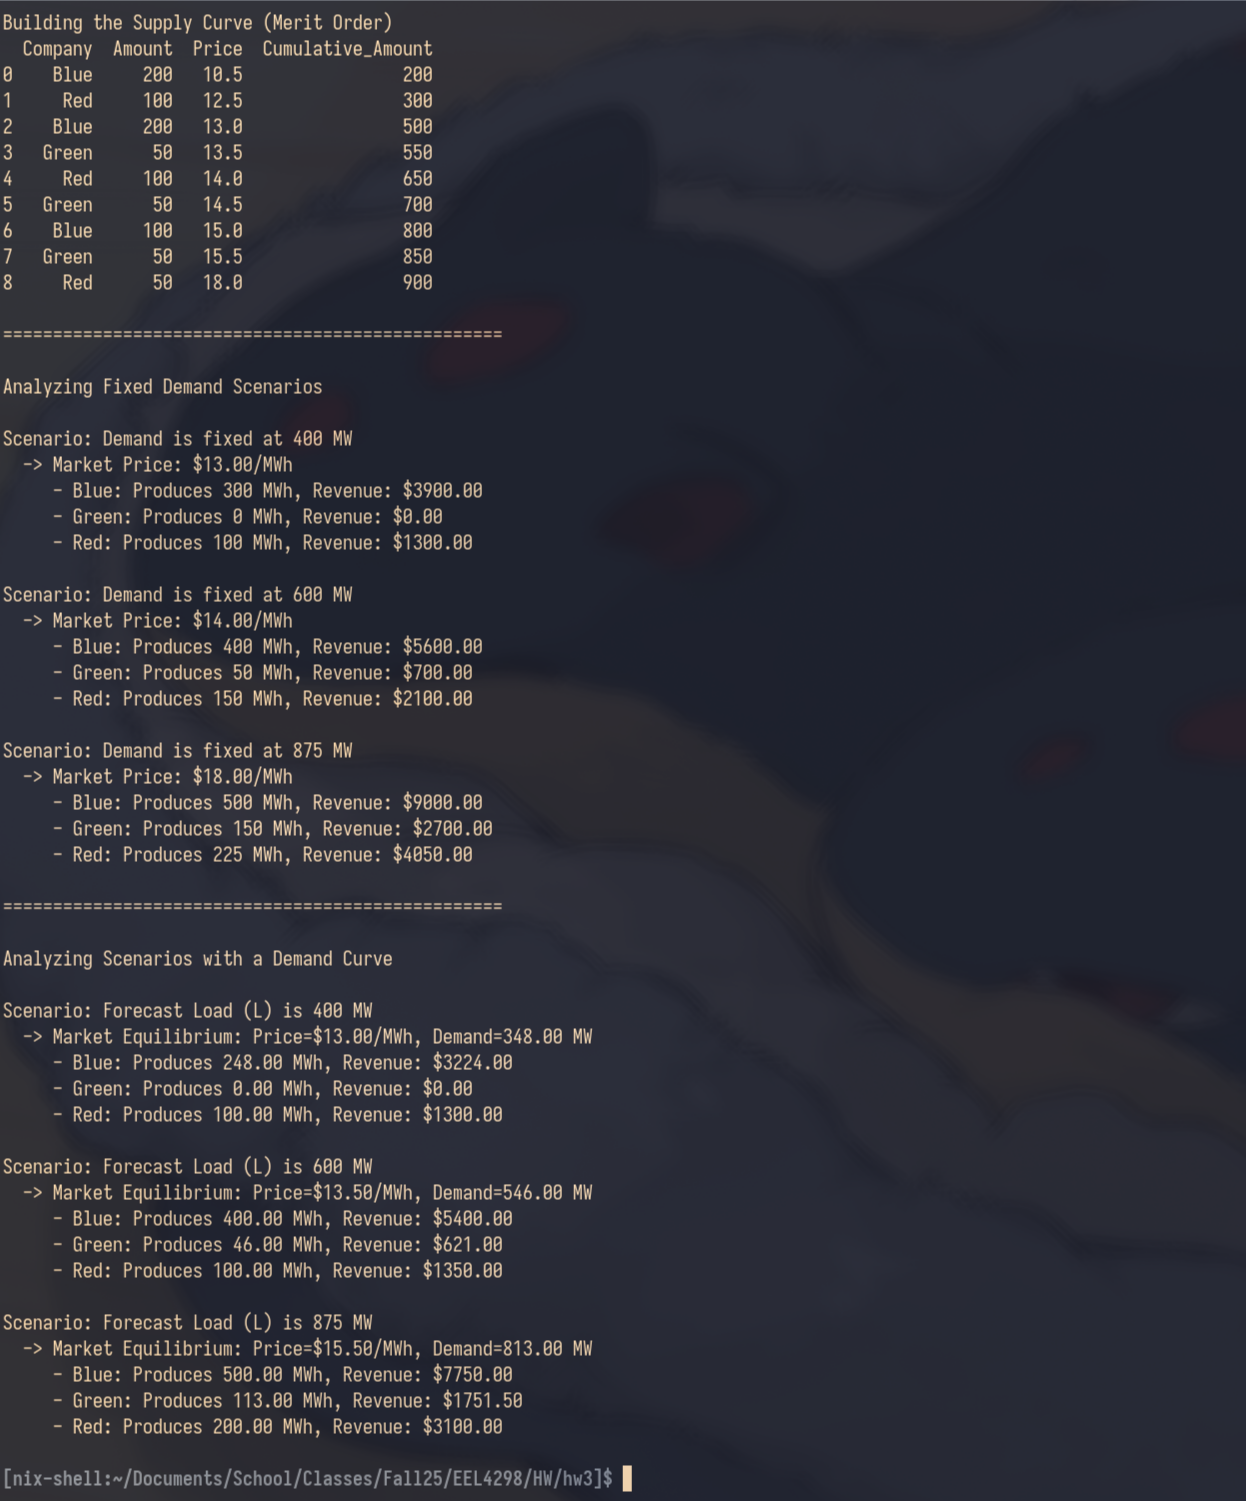
\includegraphics[width=\textwidth]{beta.png}

\end{document}
